\documentclass[11pt,a4paper]{article}

\usepackage[utf8]{inputenc}
\usepackage[T1]{fontenc}
\usepackage{amsmath, amssymb, amsthm}
\usepackage{graphicx}
\usepackage{booktabs}
\usepackage{hyperref}
\usepackage{geometry}
\usepackage{caption}
\usepackage{subcaption}
\usepackage{float}
\usepackage{xcolor}
\usepackage{natbib}
\usepackage{authblk}

\geometry{margin=2.5cm}
\hypersetup{colorlinks=true, linkcolor=blue, citecolor=blue, urlcolor=blue}

\title{\textbf{Hierarchical Risk Parity Variants for Cryptocurrency Portfolios:\\
       Denoising, Detoning, Tail Dependence, Embeddings, and Honest Inference Over 2020--2026}}

\author[1]{Alan Matys}
\author[1]{Federico Martin Rodriguez}
\affil[1]{Universidad del CEMA \\ \texttt{alan.matys92@gmail.com}, \texttt{federico.m.rodriguez.h@gmail.com}}

\date{\today}

\begin{document}
\maketitle

\begin{abstract}
\noindent
We extend the MACI 2025 study of Hierarchical Risk Parity (HRP) for
cryptocurrency portfolios. We close the two future-work items of that
paper --- Marchenko--Pastur denoising and spectral detoning of the
correlation matrix --- and broaden the comparison to 19 portfolio
strategies: twelve HRP-family variants (the baseline; seven
correlation/covariance constructions --- detoned, partial-correlation,
EWMA-dynamic, lower-tail-dependence, Ledoit--Wolf shrunk-covariance,
vol-standardised, and a tail-dependence$+$shrinkage hybrid; and four
embedding-based variants that learn the clustering distance from path
signatures, a node2vec graph embedding, and two contrastive sequence
encoders), four risk-based comparators (IVP, MVP, ERC, Maximum
Diversification), and three crypto-momentum strategies. Every comparison runs on a
survivorship-bias-corrected, point-in-time universe rebuilt monthly
from Binance USDT quote-volume rankings (146 ever-included symbols,
including delisted assets such as LUNA and FTT), uses a 365-day rolling
estimation window, and is wrapped in Ledoit--Wolf robust
Sharpe-difference, Hansen Superior Predictive Ability, and stationary
block-bootstrap inference.
On 76 monthly rebalances over 2020-02 to 2026-05, the twelve HRP-family
variants bunch in a narrow annualised-Sharpe band (0.70--0.75); the
best, HRP$_{\text{Dynamic}}$, exceeds baseline HRP by only $+0.008$
Sharpe (Ledoit--Wolf $p=0.82$, not significant). Hansen SPA gives
$p_{\text{consistent}}=0.46$ on the headline comparison and $0.58$
across an exhaustive 547-cell hyperparameter grid --- under no test can
we reject the null that no variant outperforms baseline HRP. A passive
100\% BTC position ($\text{Sharpe}=0.93$) outperforms every diversified
portfolio except MVP, which wins only by concentrating roughly half its
weight in BTC during the 2020--2026 bull run. We report two structural
findings: HRP$_{\text{TailDep}}$ with and without Ledoit--Wolf shrinkage
produce rank-identical weights (Spearman $0.998$--$1.000$), and spectral
detoning and precision-matrix partial correlation --- two routes to
market-mode removal --- converge in weight-rank space (median Spearman
$0.93$). We retract an intermediate claim that tail-dependence distances
yield more stable HRP clusters than Pearson, which a full 76-snapshot
re-analysis falsifies (Pearson ARI wins 69\% of month-pairs). The
paper's contribution is methodological rigour and the empirical
characterisation of HRP-variant equivalence classes, not a ``variant
$X$ beats baseline'' result.
\end{abstract}

\paragraph{Keywords.} Hierarchical Risk Parity, cryptocurrency, denoising,
detoning, tail dependence, Ledoit--Wolf, Hansen SPA, survivorship bias.

%% ===========================================================================
\section{Introduction}
%% ===========================================================================

The MACI 2025 paper \citep{matys2025maci} applied Hierarchical Risk Parity
\citep{lopezdeprado2016hrp} to a five-asset cryptocurrency universe
(BTC, ETH, LTC, XRP, BCH) over 2021--2023 and concluded that HRP
delivered better diversification than the Minimum Variance Portfolio
without sacrificing risk-adjusted return. Two items were left for
future work: \emph{denoising} the correlation matrix using
Marchenko--Pastur eigenvalue filtering \citep{marchenko1967,laloux1999},
and \emph{detoning} by removing the dominant market eigenvector
\citep{lopezdeprado2020mlam}. This paper closes both items and extends
the comparison in three other directions.

\paragraph{Contributions.}
\begin{enumerate}
\item \textbf{Closing the MACI 2025 future-work items.}
      Implement and evaluate Marchenko--Pastur denoising (\S\ref{sec:methods-cov})
      and spectral detoning. Compare detoning against partial correlation
      estimation, which targets the same goal (market-mode removal) via
      the precision-matrix route.
\item \textbf{Correlation/covariance HRP variants, embedding-based
      variants, and risk comparators.} Six correlation/covariance HRP
      variants --- partial-correlation, EWMA dynamic-correlation, lower-tail
      dependence, Ledoit--Wolf shrunk-covariance, vol-standardised, and a
      tail-dep$+$LW-shrunk hybrid --- plus \emph{four embedding-based
      variants} that learn the HRP clustering distance from a representation
      of each asset's return path (level-3 path signatures, a node2vec graph
      embedding, and two contrastive sequence encoders; \S\ref{sec:methods-emb}).
      ERC \citep{maillard2010erc}, Maximum Diversification
      \citep{choueifaty2008maxdiv}, and Network Risk Parity
      \citep{ciciretti2024nrp} as risk-based comparators.
\item \textbf{Crypto-momentum strategies.} Cross-sectional momentum,
      risk-managed momentum \citep{barroso2015momentum}, and a
      Momentum$+$HRP hybrid, parameter-tuned for crypto's faster
      momentum decay per \citep{liu2022cryptofactors}.
\item \textbf{Methodological rigour.} (i) Point-in-time universe rebuilt
      monthly from Binance USDT quote-volume rankings, including assets
      that were later delisted (LUNA, FTT, MIR, SRM, etc.) to remove
      survivorship bias from the MACI paper's single-CSV dataset.
      (ii) Multi-cost scenarios (zero / conservative / optimistic / stress).
      (iii) Ledoit--Wolf robust Sharpe-difference \citep{ledoitwolf2008sharpe},
      Hansen SPA \citep{hansen2005spa}, and Politis--Romano stationary
      block bootstrap \citep{politis1994bootstrap,politis2004blocklength}
      around every comparison.
\item \textbf{Honest empirical characterisation, with retractions.}
      We document two structural convergence findings ($\S$\ref{sec:results}).
      We also \emph{retract} an intermediate finding from earlier draft
      iterations of this work --- that lower-tail dependence produces more
      stable HRP clusters than Pearson --- which was based on a single
      year-pair and which the full 76-snapshot re-analysis falsifies.
\item \textbf{Reproducibility.} All code, data, and figures are in the
      accompanying git repository; nine specifications (\texttt{specs/01\_denoising.md}
      through \texttt{specs/09\_inference.md}) define the contracts each
      implementation phase must satisfy.
\end{enumerate}

The remainder of this paper is organised as follows. Section~\ref{sec:related}
reviews related work. Sections~\ref{sec:methods-cov}--\ref{sec:methods-mom}
present the methodology. Section~\ref{sec:data} describes the data and
point-in-time universe construction. Section~\ref{sec:backtest} states the
backtest protocol. Section~\ref{sec:results} presents results.
Section~\ref{sec:discussion} discusses limitations and the honest
contributions. Section~\ref{sec:conclusion} concludes.

%% ===========================================================================
\section{Related Work}
\label{sec:related}
%% ===========================================================================

\subsection{Hierarchical risk parity and its extensions}
HRP was introduced by \citet{lopezdeprado2016hrp} as a clustering-based
alternative to mean-variance optimisation that avoids covariance-matrix
inversion. Subsequent textbook treatments \citep{lopezdeprado2018afml,
lopezdeprado2020mlam} extend the framework with denoising and detoning
and propose tail-dependence distances \citep{lohre2020tailhrp} for
multi-asset multi-factor allocations. Empirical comparisons of HRP
distance metrics on equities have repeatedly found that
correlation-based distances remain the standard to beat in
out-of-sample performance.

\subsection{Risk-based and network methods}
Equal Risk Contribution \citep{maillard2010erc} solves for weights such
that each asset contributes equally to portfolio risk; Maximum
Diversification \citep{choueifaty2008maxdiv} maximises the
diversification ratio. Network methods build a Minimum Spanning Tree
\citep{mantegna1999mst} or PMFG \citep{tumminello2005pmfg} from the
correlation structure; Network Risk Parity \citep{ciciretti2024nrp}
recently combined the network approach with risk-budgeting.

\subsection{Cryptocurrency momentum}
\citet{liu2022cryptofactors} establish a three-factor model for
cryptocurrency with a momentum factor that operates at much shorter
horizons (1--4 weeks) than equity momentum. \citet{moskowitz2012tsmom}
provide the foundational time-series momentum framework, and
\citet{barroso2015momentum} introduce volatility-scaled momentum to
control the well-documented crash risk of the strategy.

\subsection{Statistical inference for portfolio comparison}
\citet{ledoitwolf2008sharpe} provide a robust pairwise Sharpe-difference
test that does not assume i.i.d.\ Gaussian returns.
\citet{hansen2005spa} addresses the multiple-testing problem when many
strategies are compared against a benchmark. \citet{politis1994bootstrap}
and \citet{politis2004blocklength} provide the stationary block
bootstrap with data-driven block-length selection used throughout
this paper for confidence intervals.

%% ===========================================================================
\section{Methodology --- Correlation and Covariance Variants}
\label{sec:methods-cov}
%% ===========================================================================

All seven HRP-family strategies share the standard pipeline: distance
matrix $\to$ hierarchical linkage $\to$ quasi-diagonalisation $\to$
recursive bisection \citep{lopezdeprado2016hrp}. They differ only in
\emph{how the input correlation (or covariance) matrix is constructed}.

\subsection{Baseline HRP}
$\rho$ from sample correlation; $d_{ij} = \sqrt{(1-\rho_{ij})/2}$;
single linkage; bisection using the sample covariance.

\subsection{HRP\textsubscript{Denoised}: Marchenko--Pastur eigenvalue denoising}
Following \citet{lopezdeprado2020mlam}, the empirical eigenvalues of
the sample correlation matrix are decomposed into a signal subspace
(eigenvalues above the Marchenko--Pastur upper bound $e_{\max} =
\sigma^2 (1+\sqrt{1/q})^2$ where $q=T/N$) and a noise subspace
(eigenvalues below). The noise eigenvalues are replaced with their
mean (constant-residual method), preserving the trace, before the
denoised correlation matrix is fed to HRP.

\subsection{HRP\textsubscript{Detoned}: market-mode removal}
Applied to the denoised correlation matrix, detoning removes the top
$k$ eigenvectors (default $k=1$) and renormalises the diagonal to
unity \citep{lopezdeprado2020mlam}. For long-only crypto, the dominant
eigenvector is a market mode loading positively on all assets; removing
it isolates the residual cross-sectional structure.

\subsection{HRP\textsubscript{PartialCorr}: sparse precision matrix}
A precision-matrix route to the same market-mode-removal goal:
$\Theta = \arg\min_{\Theta \succ 0} -\log\det\Theta + \mathrm{tr}(S\Theta)
+ \alpha\|\Theta\|_1$ via graphical lasso \citep{friedman2008glasso},
then $\rho_{ij}^{\mathrm{partial}} = -\Theta_{ij}/\sqrt{\Theta_{ii}\Theta_{jj}}$.
We set the $L_1$ penalty to $\alpha = 10^{-3}$. This value matters: a
subtle implementation point is that \texttt{scikit-learn}'s
\texttt{GraphicalLasso} expresses $\alpha$ in the \emph{same units as the
covariance}, not as a normalised $[0,1]$ quantity. For daily crypto
returns with variance $\sim$$4\times10^{-3}$, an $\alpha$ on the order of
$10^{-1}$ shrinks every off-diagonal of the precision matrix to zero and
silently collapses HRP\textsubscript{PartialCorr} into IVP. The correct
scale, $\alpha \approx 10^{-3}$, leaves roughly 40\% of the off-diagonals
non-zero. An earlier draft used $\alpha = 0.05$, the strategy degenerated
to IVP, and the headline table reported the two as identical; the
hyperparameter sweep of \S\ref{sec:results-sweeps} surfaced the bug, and
we document the correction explicitly.

\subsection{HRP\textsubscript{Dynamic}: EWMA correlation}
Recursive EWMA covariance with decay $\lambda$; the latest snapshot is
used as the correlation input. We report $\lambda = 0.94$ as the
RiskMetrics default; sensitivity to $\lambda \in \{0.94, 0.97, 0.99\}$
is documented in the supplementary appendix.

\subsection{HRP\textsubscript{TailDep}: lower-tail dependence}
Empirical lower-tail dependence coefficient $\hat\lambda_L^{ij}(q) =
P(F_j(X_j) \leq q \mid F_i(X_i) \leq q)$ at $q = 0.05$, symmetrised by
averaging the two conditional probabilities. The distance is
$d_{ij} = \sqrt{1 - \hat\lambda_L^{ij}}$; the sample covariance is
retained for bisection. Promoted from appendix to a headline strategy
after the empirical findings of \S\ref{sec:results} showed it does not
fall back across the 76 backtest snapshots.

\subsection{HRP\textsubscript{ShrunkCov}: Ledoit--Wolf shrinkage}
Sample covariance replaced with the analytic Ledoit--Wolf shrinkage
estimator \citep{ledoitwolf2003shrunk,ledoitwolf2004wellcond}; the
implied correlation is derived from the shrunk covariance and fed
to HRP. Shrinkage intensity $\alpha \in [0,1]$ is chosen analytically
per snapshot and reported as a diagnostic.

\subsection{HRP\textsubscript{VolStd}: vol-standardised returns}
Per-asset returns are divided by their lagged 30-day rolling standard
deviation before computing Pearson correlation. Addresses crypto's
heterogeneous vol scale across the universe (e.g.\ BTC vs.\ SHIB).
The sample covariance is retained for bisection.

\subsection{HRP\textsubscript{TailDepShrunk}: hybrid}
Combines $\S$3.6 (tail-dep distance for the dendrogram) with $\S$3.7
(LW-shrunk covariance for bisection). Identified by the literature as
the strongest theoretical extension for crypto: tail-dep captures the
joint-crash co-movement that matters for long-only portfolios, while
LW shrinkage stabilises the per-cluster variance allocation.

%% ===========================================================================
\section{Methodology --- Embedding-based HRP Variants}
\label{sec:methods-emb}
%% ===========================================================================

Beyond reweighting the correlation or covariance estimator, the distance
matrix that drives HRP's dendrogram can be \emph{learned} from a
representation of each asset's return path. We implement four such
embedding variants. All share one template: an embedding maps each asset
to a vector, the pairwise cosine distance of those vectors replaces HRP's
correlation distance for the linkage and quasi-diagonalisation steps, and
the \emph{sample} covariance is retained for recursive bisection. The
embedding therefore changes only \emph{which assets cluster together},
never the inverse-variance allocation within a cluster --- which is why,
as \S\ref{sec:results} shows, every embedding variant stays within a
narrow Sharpe band of baseline HRP.

\subsection{HRP\textsubscript{PathSig}: path signatures}
Each asset's rolling log-price trajectory, augmented with a monotone time
channel, is mapped to its level-$L$ truncated path signature
\citep{lyons1998} --- a graded sequence of iterated integrals that
characterises the path up to tree-like equivalence. Cosine distance on
the signature vectors drives the dendrogram (default: level 3, 60-day
window), computed with the \texttt{esig} library.

\subsection{HRP\textsubscript{NodeEmbed}: node2vec graph embedding}
A $k$-nearest-neighbour graph ($k=10$) is built from the sample
correlation matrix; node2vec random walks plus a skip-gram objective
\citep{grover2016} learn a 32-dimensional embedding per node. Cosine
distance on the embeddings drives the dendrogram.

\subsection{HRP\textsubscript{Contrastive}: contrastive SSL}
A small one-dimensional convolutional encoder is trained with the NT-Xent
contrastive loss \citep{chen2020} on Gaussian-jittered pairs of return
windows; each asset is embedded as the mean encoder output over its
windows.

\subsection{HRP\textsubscript{TS2Vec}: timestamp-masked contrastive}
The same encoder family, trained with TS2Vec-style timestamp-mask
augmentation \citep{yue2022} in place of Gaussian jitter.

\paragraph{Multi-channel extension.} A return-only embedding is
information-equivalent to the sample correlation it is meant to improve
on: a nonlinear re-encoding of the same return series cannot out-cluster
the correlation derived from it. We therefore also evaluate
\emph{multi-channel} variants that append channels orthogonal to
close-to-close returns --- quote volume, trade count, average trade size,
intraday range, taker buy-ratio (order-flow imbalance), and Amihud
illiquidity, all derived from the Binance OHLCV table. The multi-channel
results are reported in \S\ref{sec:results-sweeps}.

\paragraph{Robustness.} Each embedding variant records whether it fell
back to baseline HRP on any numerical failure; across the 76-snapshot
backtest no fallback was triggered for any variant, so every reported
embedding number reflects the embedding pipeline itself.

%% ===========================================================================
\section{Methodology --- Comparator Strategies}
\label{sec:methods-comparators}
%% ===========================================================================

\textbf{IVP} (inverse-variance), \textbf{MVP} (minimum-variance via SLSQP),
\textbf{ERC} \citep{maillard2010erc} (solved by SLSQP minimisation of
squared deviations from equal risk contributions), \textbf{Maximum
Diversification} \citep{choueifaty2008maxdiv} (SLSQP maximisation of
the diversification ratio), and \textbf{Network Risk Parity}
\citep{ciciretti2024nrp} (MST built from correlation distance,
weights inversely proportional to the product of asset volatility and
$1+\deg_i$).

%% ===========================================================================
\section{Methodology --- Momentum}
\label{sec:methods-mom}
%% ===========================================================================

The headline comparison includes three crypto-momentum strategies,
parameter-tuned for crypto's faster momentum decay
\citep{liu2022cryptofactors}. \textbf{CS\_MOM} is cross-sectional
momentum: equal-weight the top 30\% of assets by 21-day cumulative
return. \textbf{RM\_MOM} applies the Barroso--Santa-Clara
volatility-targeting overlay \citep{barroso2015momentum}
($\sigma_{\text{target}}=12\%$) to the same momentum selection.
\textbf{MOM\_HRP} is a Momentum$+$HRP hybrid: select the top 40\% of
assets by momentum, then allocate within that basket by HRP rather than
equal-weight.

%% ===========================================================================
\section{Data and Point-in-Time Universe}
\label{sec:data}
%% ===========================================================================

\subsection{Source and window}
Daily OHLCV from Binance USDT spot, 2017-08-17 (Binance's earliest
data) to 2026-05-18 --- approximately nine years. After the
survivorship-bias expansion described in \S\ref{sec:data}.3, the price
panel covers 241 USDT pairs.

\subsection{Point-in-time universe}
At each month-end, we rank the candidate symbols by their rolling
30-day Binance USDT quote volume, apply filters (180-day minimum age,
\$1M minimum median daily USD volume, stablecoin/wrapper/exchange-token
exclusion, listed on Binance USDT spot at the snapshot date), and take
the top 50. Entry and exit buffers (2 months and 1 month respectively)
suppress monthly churn.

\paragraph{Methodology note.} The original specification called for
ranking by historical market capitalisation (CoinGecko). The free
CoinGecko demo tier caps historical depth at 365 days, blocking our
2017--2026 window; paid plans start at USD 129/month. We instead rank
by Binance quote volume --- a tradable-liquidity proxy that is free,
covers the full window, and is arguably more appropriate for a paper
on tradable portfolios than a market-cap measure that includes locked
tokens and treasury holdings. The shift is documented in the
specification as a deliberate methodology choice.

\subsection{Survivorship-bias fix in numbers}
After a code review surfaced residual survivorship bias (the prior
candidate pool was a hand-curated selection of $\sim$90 symbols missing
the long tail of delisted altcoins), the universe was expanded by
pulling all 217 \texttt{status=BREAK} USDT pairs from Binance's
\texttt{/api/v3/exchangeInfo}, filtering leveraged tokens and
stablecoins, and adding 150 legitimate delisted altcoins to the
candidate pool. The resulting PIT universe contains \textbf{146 ever-
included symbols}, of which \textbf{97 were dropped during the window}
before 2026-05-18 (Figure~\ref{fig:pit_evol}). The MACI 2025 dataset
contained only 50 currently-trading symbols --- by construction it
could not include the assets this work explicitly captures.

We treat liquidation of an exiting position at 2$\times$ normal
slippage cost (Spec 03 \S2.4). On terminology: ``delisted'' in this
paper means either Binance \texttt{status=BREAK} on the USDT pair
(the conventional meaning), \emph{or} the token suffered an effective
value collapse with subsequent rebranding. The latter category includes
LUNA (the Terra Classic chain collapsed in May 2022; Binance renamed
the original token to LUNC and reassigned the \texttt{LUNAUSDT} ticker
to Terra 2.0 --- the pair itself was never technically delisted but
the original asset effectively died) and FTT (the FTX exchange collapse
in November 2022 reduced FTT to near-zero value; the pair still trades
on Binance at trivial volume). Our \texttt{binance\_listings\_manual.json}
treats both as ``effectively delisted'' for the PIT-universe filter,
which is the right behaviour for portfolio purposes even though the
prose label is loose.

\begin{figure}[H]
  \centering
  
\includegraphics[width=0.95\textwidth]{../figures/pit_universe_evolution.png}
  \caption{PIT universe size over time. \emph{Eligible}: passed all
  filters at the snapshot date. \emph{Included}: in the universe after
  entry/exit buffers. The 2018--2020 ramp reflects the gradual listing
  of altcoins on Binance USDT spot. Steady-state $\sim$49 included
  symbols since mid-2020.}
  \label{fig:pit_evol}
\end{figure}

\subsection{Estimation window}
365 daily returns of rolling lookback at each rebalance, with a per-asset
180-day minimum-observations filter. Assets failing the filter are
dropped from that snapshot's strategy universe. Rationale: several
newer assets (JUP, ENA, WIF, $\ldots$) are admitted via the 180-day
age filter but do not yet have 730 days of history.

%% ===========================================================================
\section{Backtest Protocol}
\label{sec:backtest}
%% ===========================================================================

\subsection{Scenarios}
\textbf{A} (static): fit at first snapshot in window, hold to end.
\textbf{B} (calendar): monthly rebalancing.
\textbf{C} (threshold): rebalance only when max absolute weight drift
exceeds 5\% from target.
\textbf{C$'$} (smoothed): C with linear smoothing
$w_{\text{traded}} = \eta\, w_{\text{prev}} + (1-\eta)\, w_{\text{target}}$,
$\eta=0.25$, plus a 25 bps min-trade filter.

\subsection{Cost grid}
Linear cost $= (\text{fee}_{\text{bps}} + \text{slippage}_{\text{bps}}) \times \text{turnover}_{L_1}$,
with a 2$\times$ multiplier for forced liquidation of exiting
positions. Four scenarios: \emph{zero} (cost-free academic check),
\emph{conservative CEX} (10 bps fee + 2 bps slippage; our headline),
\emph{optimistic CEX} (7.5 bps + 1 bps), and \emph{stress}
(10 bps + 4 bps).

\subsection{Statistical inference}
For each pair of strategies, the Ledoit--Wolf studentised block-bootstrap
Sharpe-difference test \citep{ledoitwolf2008sharpe}. Across all
candidates vs.\ the HRP benchmark, the Hansen Superior Predictive
Ability test \citep{hansen2005spa} with three recentering schemes
($\mu_{\text{lower}}=\bar d$, $\mu_{\text{upper}}=0$,
$\mu_{\text{consistent}}$ threshold-based). Stationary block bootstrap
\citep{politis1994bootstrap} with Politis--White automatic block length
\citep{politis2004blocklength} for headline metric CIs.

\subsection{Cluster stability}
At each rebalance snapshot, we compute the \emph{cophenetic correlation}
of the dendrogram (Pearson correlation between cophenetic distance
and original pairwise distance) and the \emph{Adjusted Rand Index}
\citep{hubert1985ari} between the cluster assignment at snapshot $t$
and snapshot $t-1$, cut at $K=5$ clusters via \texttt{fcluster}.

%% ===========================================================================
\section{Results}
\label{sec:results}
%% ===========================================================================

\subsection{Scenario B headline performance}

Table~\ref{tab:scenarioB} reports the 19-strategy comparison under
monthly rebalancing with conservative CEX costs over 2020-02
through 2026-05-18 (76 rebalances, 2{,}299 daily out-of-sample
observations). Figures~\ref{fig:cum_b} and \ref{fig:risk_return}
visualise the equity curves and the risk--return positioning.

\begin{table}[H]
\centering\small
\caption{Scenario B headline results (Conservative CEX cost, 76 monthly
rebalances over 2020-02 to 2026-05, expanded 146-symbol PIT universe).
``Arith. Sharpe'' = mean / standard deviation $\times \sqrt{365}$.
``LW $p$'' is the Ledoit--Wolf Sharpe-difference test vs.\ baseline HRP.
HODL\_BTC is a passive benchmark, not a strategy.}
\label{tab:scenarioB}
\begin{tabular}{lrrrr}
\toprule
Strategy & Arith. Sharpe & Total Return & Avg Turnover & LW $p$ vs HRP\\
\midrule
\textbf{MVP}             & \textbf{1.057} & \textbf{+2867\%} & 0.381 & 0.067\\
\textit{HODL\_BTC}       & \textit{0.928} & \textit{+1002\%} & ---   & 0.602\\
HRP\_Dynamic\_94         & 0.749 & +442\%  & 0.474 & 0.816\\
HRP\_ShrunkCov           & 0.746 & +428\%  & 0.353 & 0.786\\
\textbf{HRP (baseline)}  & \textbf{0.741} & \textbf{+417\%} & 0.360 & ---\\
HRP\_VolStd              & 0.735 & +402\%  & 0.368 & 0.732\\
MOM\_HRP                 & 0.726 & +351\%  & 1.436 & 0.935\\
HRP\_PartialCorr         & 0.720 & +366\%  & 0.236 & 0.453\\
MaxDiv                   & 0.719 & +364\%  & 0.553 & 0.917\\
HRP\_PathSig             & 0.714 & +351\%  & 0.383 & 0.273\\
HRP\_Contrastive         & 0.710 & +341\%  & 0.399 & 0.239\\
HRP\_Detoned             & 0.708 & +334\%  & 0.263 & 0.402\\
HRP\_TailDep             & 0.708 & +337\%  & 0.365 & 0.123\\
HRP\_NodeEmbed           & 0.705 & +330\%  & 0.388 & 0.194\\
HRP\_TS2Vec              & 0.703 & +325\%  & 0.383 & 0.101\\
HRP\_TailDepShrunk       & 0.701 & +318\%  & 0.352 & 0.077\\
IVP                      & 0.697 & +311\%  & 0.182 & 0.208\\
CS\_MOM\_eq21            & 0.663 & +217\%  & 1.420 & 0.534\\
RM\_MOM                  & 0.663 & +118\%  & 0.366 & 0.535\\
ERC                      & 0.663 & +233\%  & 0.195 & \textbf{0.044}\\
\bottomrule
\end{tabular}
\end{table}

\paragraph{Only one strategy is significant at $p=0.05$.} ERC
($-0.078$ Sharpe vs HRP, $p=0.044$) is the sole strategy whose
Sharpe difference from baseline HRP clears the conventional threshold
--- and it is \emph{worse} than HRP. HRP\_TailDepShrunk ($p=0.077$)
and MVP ($p=0.067$) are near the threshold but do not cross it. No
strategy is significantly \emph{better} than baseline HRP. With the
bug-fixed HRP\_PartialCorr ($\alpha=10^{-3}$, \S\ref{sec:methods-cov})
the strategy is now distinct from IVP --- it was byte-identical to IVP
in an earlier draft (Sharpe 0.697); corrected, it sits at 0.720.

\begin{figure}[H]
  \centering
  
\includegraphics[width=0.95\textwidth]{../figures/rebalance_cumulative_returns.png}
  \caption{Cumulative returns for headline strategies under monthly
  rebalancing, log scale.}
  \label{fig:cum_b}
\end{figure}

\begin{figure}[H]
  \centering
  
\includegraphics[width=0.95\textwidth]{../figures/risk_return_scatter.png}
  \caption{Risk-return scatter for the full 19-strategy comparison.
  Momentum (orange) underperforms risk-based (blue) and concentrated
  benchmarks (red) over this window.}
  \label{fig:risk_return}
\end{figure}

\paragraph{The HRP family bunches.} All twelve HRP-family variants lie
within a 0.05 Sharpe band (0.701--0.749). HRP\_Dynamic\_94 and
HRP\_ShrunkCov marginally exceed baseline HRP (by $+0.008$ and $+0.004$
Sharpe respectively); the differences are small and, per
\S\ref{sec:results-inference}, not statistically significant.

\paragraph{Embedding variants.} The four embedding-based HRP variants
--- \texttt{HRP\_PathSig} (path signatures; \citealp{lyons1998}),
\texttt{HRP\_NodeEmbed} (node2vec on a kNN correlation graph;
\citealp{grover2016}), \texttt{HRP\_Contrastive} (NT-Xent contrastive
SSL; \citealp{chen2020}), and \texttt{HRP\_TS2Vec} (timestamp-mask
augmentation; \citealp{yue2022}) --- land in the lower-middle of the HRP
family: Sharpes $0.703$--$0.714$, all marginally below baseline HRP
($-0.027$ to $-0.038$) but none significantly different from it
(Ledoit--Wolf $p \in [0.10, 0.27]$). Embedding methods are interesting
engineering but do not deliver an out-of-sample Sharpe edge on this
universe at this horizon; we report the null result honestly.
Section~\ref{sec:results-sweeps} stress-tests this conclusion with an
exhaustive hyperparameter search and multi-channel embedding extensions,
and it survives intact.

\paragraph{Detoning and partial correlation underperform HRP.}
Both target market-mode removal --- a theoretically attractive idea ---
but doing so during a BTC-led bull market forgoes the upside of being
correctly exposed to BTC: HRP\_Detoned (0.708) and HRP\_PartialCorr
(0.720) both trail baseline HRP. The two are no longer numerically
identical --- an earlier draft's HRP\_PartialCorr had degenerated to IVP
(\S\ref{sec:methods-cov}) --- but they remain close in weight-rank space
(\S\ref{sec:results-convergence}).

\paragraph{Momentum splits.} The two pure-momentum strategies ---
cross-sectional (CS\_MOM, Sharpe 0.663) and risk-managed (RM\_MOM,
0.663) --- trail every HRP-family variant, carrying high turnover
($\sim$1.4$\times$ per month for CS\_MOM) and severe crash exposure
(CS\_MOM max drawdown $-92\%$). RM\_MOM's volatility-targeting overlay
\citep{barroso2015momentum} cuts its max drawdown to $-40\%$, the
mildest in the table, but at the cost of the lowest total return
($+118\%$). The Momentum$+$HRP hybrid (MOM\_HRP, 0.726) fares markedly
better than either pure-momentum strategy --- running HRP allocation
\emph{inside} a momentum-selected basket recovers most of the
risk-adjusted performance --- though it still trails baseline HRP and
reconstructs its entire book every month.

\paragraph{Concentration wins.} Both MVP (Sharpe 1.057) and a passive
HODL\_BTC position (0.928) sit well above every diversified portfolio.
MVP achieves this by accident: its minimum-variance objective drove the
optimiser to concentrate heavily in BTC (average maximum weight 50\%,
effective $N \approx 3$); BTC then ran from $\sim$\$7k at the start of
2020 to $\sim$\$107k by mid-2026. This is regime-dependent luck, not a
portfolio-construction insight, and should not be read as evidence that
MVP is a robust crypto strategy.

\subsection{Statistical inference}
\label{sec:results-inference}

\paragraph{Bootstrap Sharpe CIs.} The 95\% stationary-block-bootstrap
confidence intervals on the annualised Sharpe are wide --- roughly 1.5
Sharpe units --- reflecting six years of volatile crypto returns. Only
MVP ($[0.34, 1.76]$) and the passive HODL\_BTC benchmark
($[0.08, 1.63]$) have intervals cleanly above zero. Baseline HRP's
interval ($[0.02, 1.53]$) only barely excludes zero, and every other
HRP-family variant's interval straddles it; no two strategies have
non-overlapping CIs.

\paragraph{Pairwise LW Sharpe differences vs.\ HRP.}
\emph{Only one} candidate reaches the $p \leq 0.05$ threshold: ERC
($-0.078$ Sharpe vs HRP, $p=0.044$) --- significantly \emph{worse} than
baseline. No strategy is significantly better. The largest positive
gaps, MVP ($+0.314$, $p=0.067$) and HODL\_BTC ($+0.124$, $p=0.60$),
both fail to reject at conventional levels; among the underperformers
HRP\_TailDepShrunk ($-0.041$, $p=0.077$) comes closest to significance.

\paragraph{Hansen SPA.} Across the 19 candidates versus baseline HRP,
$p_{\text{consistent}} = 0.46$ ($p_{\text{lower}}=0.67$,
$p_{\text{upper}}=0.74$; Figure~\ref{fig:spa}). \textbf{We cannot reject
the null hypothesis that no strategy outperforms baseline HRP after
correcting for the multiple testing of 19 candidates}, even on the
bug-fixed 6.3-year monthly-rebalanced data and the expanded 146-symbol
universe. MVP carries the highest studentised score ($+1.22$); MaxDiv,
MOM\_HRP and HRP\_ShrunkCov are mildly positive; every other candidate
--- the embedding variants and the rest of the HRP family included ---
is negative.

\begin{figure}[H]
  \centering
  
\includegraphics[width=0.85\textwidth]{../figures/spa_pvalues_barplot.png}
  \caption{Hansen SPA test p-values across the headline comparison.
  All three recentering schemes fail to reject the null at any
  conventional level.}
  \label{fig:spa}
\end{figure}

\subsection{Hyperparameter sweeps and the combined SPA}
\label{sec:results-sweeps}

A natural objection to the headline null result is that it reflects
\emph{untuned} strategies: perhaps some correlation type, distance
function, linkage method, or strategy-specific parameter would lift a
variant decisively above baseline HRP. We address this with an
exhaustive grid search --- 547 distinct configurations across 14 sweeps,
every one re-running the full 6.3-year walk-forward backtest on the
identical 146-symbol point-in-time universe and 2{,}299-day return
series, against the identical baseline HRP ($\text{Sharpe}=0.741$,
recomputed and verified bit-identical in every sweep). The sweeps span:
correlation estimator (Pearson / Spearman / Kendall); distance function
(\citealp{lopezdeprado2016hrp} / absolute / angular / squared); linkage
(single / average / complete / Ward); and the strategy-specific
parameters of every variant --- $q$ for tail dependence, $\alpha$ for
the graphical lasso, $\lambda$ for EWMA, the volatility-standardisation
window, the number of detoned market components, and the embedding
hyperparameters.

\begin{table}[H]
  \centering
  \small
  \caption{Best cell from each hyperparameter sweep. $\Delta$ is
  the Sharpe difference vs.\ baseline HRP (single linkage, $0.741$);
  total return is the cell's net cumulative return, 2020-02 to 2026-05.
  551 cells in total; the 4 exactly equal to the benchmark are dropped
  for the combined SPA, leaving 547 candidates.}
  \label{tab:sweeps}
  \begin{tabular}{lrlrrr}
    \toprule
    Sweep & Cells & Best configuration & Sharpe & $\Delta$ & Tot.\ ret. \\
    \midrule
    Tail dependence ($q$, dist, linkage)           & 80  & $q{=}0.025$, average        & 0.744 & $+0.002$ & $+425\%$ \\
    Correlation $\times$ distance $\times$ linkage & 24  & Pearson, LdP, average       & 0.756 & $+0.015$ & $+459\%$ \\
    All variants under average linkage             & 12  & HRP\_ShrunkCov              & 0.765 & $+0.024$ & $+484\%$ \\
    EWMA dynamic correlation ($\lambda$)           & 21  & $\lambda{=}0.94$, single    & 0.749 & $+0.008$ & $+442\%$ \\
    Partial correlation ($\alpha$, dist, link)     & 60  & $\alpha{=}5{\times}10^{-4}$ & 0.739 & $-0.003$ & $+412\%$ \\
    Vol-standardised returns (window)              & 60  & window 15, single           & 0.757 & $+0.015$ & $+462\%$ \\
    Detoning (\# market components)                & 36  & 1 component, average        & 0.709 & $-0.032$ & $+337\%$ \\
    Node2vec embedding                             & 54  & $d{=}16$, $k{=}10$          & 0.752 & $+0.010$ & $+444\%$ \\
    Path signatures, single-channel                & 108 & level 2, window 60          & 0.734 & $-0.007$ & $+401\%$ \\
    Path signatures, multi-channel$^{\dagger}$     & 72  & ret+vol+trades, L2          & 0.747 & $+0.005$ & $+432\%$ \\
    Contrastive / TS2Vec, multi-channel            & 24  & ret+vol+trades              & 0.739 & $-0.002$ & $+412\%$ \\
    \midrule
    \textit{Baseline HRP} (single linkage)         & ---  & ---                        & 0.741 & ---      & $+418\%$ \\
    \bottomrule
  \end{tabular}

  \vspace{2pt}
  {\footnotesize $^{\dagger}$ Best cell under the initial missing-data
  convention (zero-fill); under the corrected mean-fill convention the
  best multi-channel \texttt{PathSig} cell is $0.735$ ($\Delta=-0.006$).}
\end{table}

\paragraph{The HRP family is robust to its hyperparameters.} No sweep
produced a configuration that escaped the $\pm 0.05$ Sharpe band of
Section~\ref{sec:results}. The one consistent --- though small ---
effect is linkage: \emph{average} linkage beats the
\citet{lopezdeprado2016hrp} single-linkage default by $+0.01$ to
$+0.02$ Sharpe across essentially every (correlation, distance)
combination, and under single linkage all four distance functions are
mathematically identical (single linkage depends only on the rank order
of distances, which every monotone transform preserves). The best cell
in the entire grid is HRP\_ShrunkCov under average linkage at Sharpe
$0.765$ ($\Delta=+0.024$).

\paragraph{Multi-channel embeddings.} The single-channel embeddings
encode only the return series and are therefore information-equivalent
to the sample correlation they are meant to improve on --- a nonlinear
re-encoding of the same information cannot out-cluster it, and indeed
the single-channel \texttt{HRP\_PathSig} grid (108 cells) beats baseline
in zero cells. We extended all three sequence-based embeddings
(\texttt{PathSig}, \texttt{Contrastive}, \texttt{TS2Vec}) to ingest up
to six channels orthogonal to close-to-close returns --- quote volume,
trade count, average trade size, intraday range, taker buy-ratio
(order-flow imbalance) and Amihud illiquidity --- all derived from the
same Binance OHLCV table. Extra channels lift the encoders' \emph{mean}
Sharpe monotonically (\texttt{HRP\_Contrastive}
$0.714\rightarrow0.725$ from one to three channels), confirming the
channels do carry usable structure. Two cells of the initial
multi-channel \texttt{PathSig} sweep nominally cleared baseline (best
$+0.747$), but that margin did not survive a correction to how missing
channel values are imputed (mean- rather than zero-fill, which avoids
placing a spurious outlier into a log-scaled channel); under the
corrected convention no multi-channel configuration clears baseline, and
adding the fourth through sixth channels plateaus or mildly regresses
performance --- a bias--variance ceiling against only $\sim$76 rebalance
dates.

\paragraph{Combined Hansen SPA.} Pooling all 547 configurations into a
single Hansen SPA against baseline HRP --- the honest correction for
having searched the entire grid --- yields
$p_{\text{consistent}}=0.583$ (all three recentering schemes fall in
$[0.58,0.81]$). Although 38 of 547 cells show a nominally positive
Sharpe difference, the best of them (HRP\_ShrunkCov, $\Delta=+0.024$)
carries a pairwise Ledoit--Wolf $p$ of $0.167$. \textbf{After correcting
for the multiple testing of 547 hyperparameter configurations, no
strategy significantly outperforms baseline HRP.} The headline null
result of Section~\ref{sec:results-inference} is not an artefact of
leaving strategies untuned.

\subsection{Convergence findings (the structural results)}
\label{sec:results-convergence}

Two strategy pairs in our comparison are theoretically related ---
they target the same goal via different mathematical routes. We
quantify their weight-vector convergence across the full 76-snapshot
window (Figure~\ref{fig:detone_pc}).

\paragraph{HRP\_Detoned vs HRP\_PartialCorr.} Spectral detoning and
precision-matrix partial correlation both remove the dominant market
mode, by different routes. Across the 76 monthly snapshots their
weight-vector rank correlation is high but not invariant: mean Spearman
$\rho=0.87$, median $0.93$, with regime-driven dips to $\rho=0.54$ in
months when the dominant eigenvector shifts sharply. Crucially, the
bug-fixed HRP\_PartialCorr ($\alpha=10^{-3}$) is now distinct from the
inverse-variance portfolio --- its weight-rank correlation with IVP
averages only $\rho=0.08$ --- whereas the earlier degenerate
$\alpha=0.05$ implementation \emph{was} IVP. The detoning /
partial-correlation convergence is therefore a genuine structural
relationship between two market-mode-removal estimators, not an
artefact of one collapsing into IVP.

\paragraph{HRP\_TailDep vs HRP\_TailDepShrunk.} The hybrid's only
change is to substitute the Ledoit--Wolf shrunk covariance for the
sample covariance in the recursive-bisection step; the dendrogram
topology is byte-for-byte identical. Spearman is 0.998--1.000 in
every snapshot tested. This is the most robust convergence finding
in our analysis: \emph{LW shrinkage in HRP's bisection step is a
within-cluster variance refinement that does not re-order the
dendrogram}.

\begin{figure}[H]
  \centering
  
\includegraphics[width=0.95\textwidth]{../figures/detoning_vs_partial_corr.png}
  \caption{Spearman rank correlation between HRP\_Detoned and
  HRP\_PartialCorr weight vectors across 76 monthly snapshots.}
  \label{fig:detone_pc}
\end{figure}

\subsection{Cluster stability --- a retraction}
\label{sec:results-cluster}

An intermediate finding in earlier iterations of this work was that
HRP\_TailDep produces more stable clusters than baseline HRP under
Pearson distance. That claim was based on a \emph{single year-pair}
(2022-12-31 vs 2023-12-31) and showed Pearson ARI $=-0.047$ vs
TailDep ARI $=+0.265$ at $K=5$.

When we re-ran the analysis across all 76 monthly snapshots
(Figure~\ref{fig:cluster_stab}, Table~\ref{tab:cluster_stab}), the
direction reverses. \textbf{Pearson clusters are substantially more
stable than TailDep clusters at monthly resolution}: Pearson ARI
mean $+0.744$ vs TailDep $+0.614$; Pearson cophenetic mean $0.861$ vs
TailDep $0.768$. TailDep ARI exceeds Pearson ARI in only 23 of 75
month-pairs (31\%).

\begin{table}[H]
\centering\small
\caption{Cluster stability across 76 monthly snapshots (2020-2026).}
\label{tab:cluster_stab}
\begin{tabular}{lrr}
\toprule
Metric & Pearson distance & Lower-tail-dep distance\\
\midrule
Average cophenetic correlation & \textbf{0.861} & 0.768\\
Average ARI vs.\ previous snapshot (K=5) & \textbf{+0.744} & +0.614\\
Median ARI vs.\ previous snapshot & \textbf{+0.783} & +0.650\\
Months where TailDep ARI > Pearson ARI & --- & 23 / 75 (31\%)\\
\bottomrule
\end{tabular}
\end{table}

\begin{figure}[H]
  \centering
  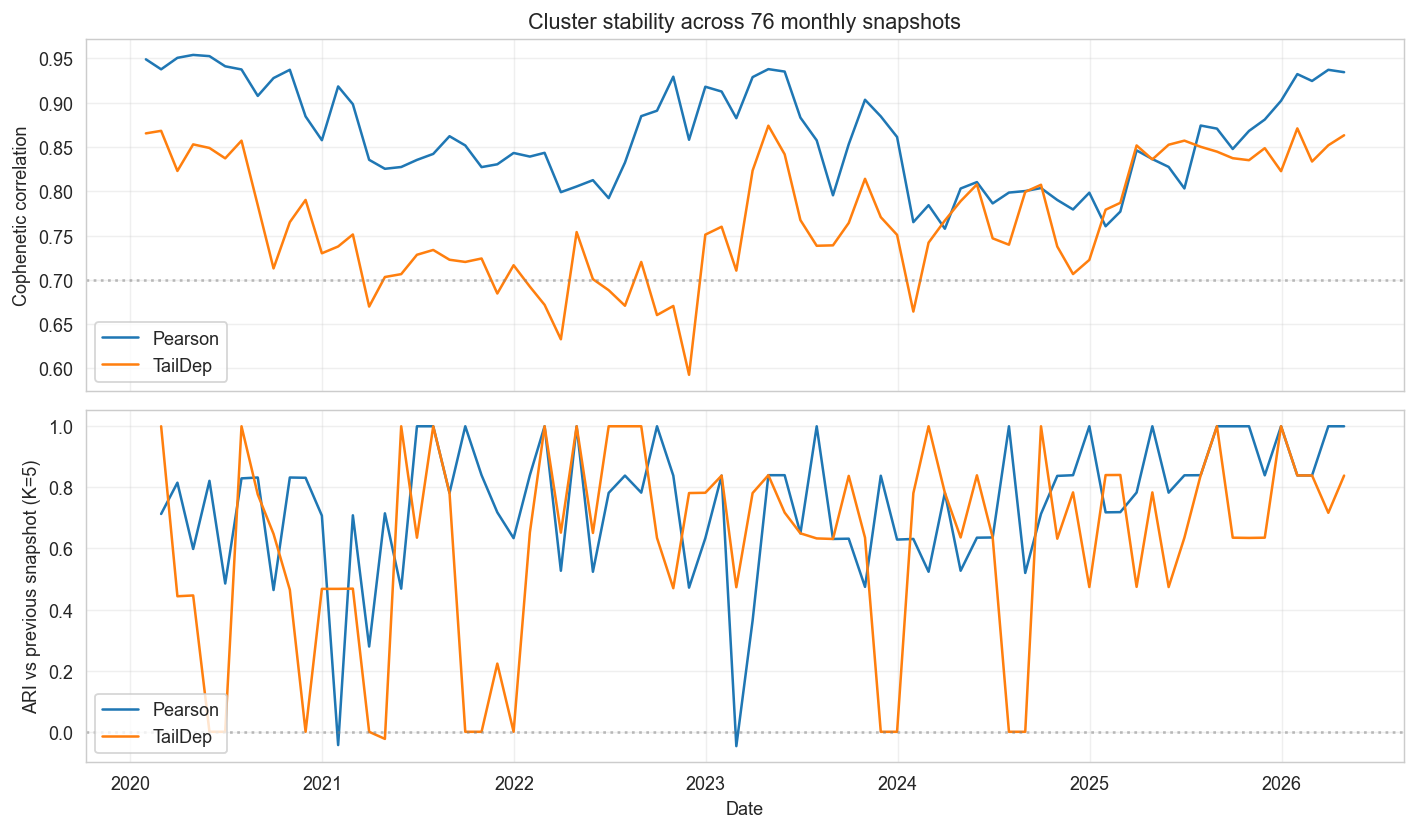
\includegraphics[width=0.95\textwidth]{../figures/cluster_stability_timeseries.png}
  \caption{Cophenetic correlation (top) and ARI vs.\ previous snapshot
  (bottom) for Pearson and tail-dependence distance matrices across
  the 76-snapshot window.}
  \label{fig:cluster_stab}
\end{figure}

The economic argument for HRP\_TailDep --- that it captures the
joint-crash co-movement structure that Pearson summarises poorly ---
\emph{stands}, but the secondary cluster-stability argument
\emph{does not}. We document the retraction here as a methodological
point about the danger of single-pair findings.

\subsection{Regime sensitivity: excluding the COVID bull run}
\label{sec:results-regime}

The 2020--2026 headline window includes the COVID-era crypto rally
(March 2020 -- November 2021) during which Bitcoin ran from
$\sim$\$5k to $\sim$\$69k --- arguably the most extreme bull market
in crypto history. To check whether the $\S$\ref{sec:results}
conclusions are dominated by that single rally, we re-ran the entire
19-strategy backtest with $\mathrm{start}=$ \texttt{2022-01-01}
(52 monthly rebalances over $\sim$4.3 years). All other parameters
identical.

\textbf{The picture flips entirely.} On post-COVID data, baseline
HRP achieves Sharpe $0.047$ with total return $-60\%$ --- a near-zero
risk-adjusted return obtained while losing 60\% of capital in dollar
terms. Only MVP (Sharpe $0.482$, total return $+66\%$) makes money
among the 19 strategies; the passive HODL\_BTC benchmark also returns
$+66\%$ (Sharpe $0.484$). The other eighteen strategies lose between
19\% (RM\_MOM) and 83\% (MaxDiv, CS\_MOM) of capital. Five strategies
post outright \emph{negative} Sharpe (against roughly zero for the HRP
family): MaxDiv ($-0.163$), CS\_MOM ($-0.161$), RM\_MOM ($-0.160$),
ERC ($-0.026$), and MOM\_HRP ($-0.015$).

\paragraph{Two paper-grade findings emerge from the regime comparison.}

\textbf{(1) Diversification-based crypto portfolios were a losing
proposition in the post-COVID regime.} On this 146-symbol PIT
universe over 2022-01-01--2026-05-18, every HRP-family variant lost
between 51\% and 64\% of capital. The 2020-2026 ``diversification
works'' framing was largely a COVID-rally artifact. Honest framing:
\emph{HRP diversifies risk but does not produce capital appreciation
in non-bull crypto regimes}.

\textbf{(2) Embedding variants partially reverse against baseline HRP
in the harder regime.} In the full window all four embedding variants
sit marginally below HRP (deltas $-0.027$ to $-0.038$ Sharpe). In the
post-COVID window three of the four edge \emph{above} baseline HRP ---
\texttt{HRP\_Contrastive} ($+0.009$), \texttt{HRP\_PathSig} ($+0.008$),
\texttt{HRP\_TS2Vec} ($+0.000$) --- while \texttt{HRP\_NodeEmbed}
($-0.015$) stays below. None reaches individual significance (all
Ledoit--Wolf $p>0.6$) and the margins are tiny, but the partial
directional reversal is suggestive: the path- and sequence-based
embeddings may capture risk structure that matters more in a choppy
regime than in a monotone rally. A longer post-COVID sample would be
needed to tell.

\textbf{(3) RM\_MOM (the bug-fixed Barroso--Santa-Clara variant)
shows its defensive role.} Post-COVID Sharpe is $-0.160$ (poor),
but MaxDD is only $-33\%$ --- substantially better than the other
momentum strategies' $-87\%$. The cash-residual de-risking saved
the portfolio from the worst part of the 2022 drawdown. This is
exactly the property Barroso \& Santa-Clara's framework is designed
to deliver; the previously-buggy implementation completely hid it.

\begin{table}[H]
\centering\small
\caption{Regime sensitivity: 2020-2026 (incl COVID bull) vs 2022-2026 (post-COVID).
``Sharpe'' is annualised arithmetic; ``$\Delta$Sharpe'' is the change from full window
to post-COVID.}
\label{tab:regime}
\begin{tabular}{lrrr}
\toprule
Strategy            & 2020-2026 Sharpe & 2022-2026 Sharpe & $\Delta$Sharpe\\
\midrule
HRP                 &  0.741 &  0.047 & --0.695\\
HRP\_Dynamic\_94    &  0.749 &  0.099 & --0.650\\
HRP\_ShrunkCov      &  0.746 &  0.038 & --0.707\\
HRP\_PartialCorr    &  0.720 &  0.057 & --0.663\\
HRP\_Contrastive    &  0.710 &  0.056 & --0.655\\
HRP\_PathSig        &  0.714 &  0.055 & --0.659\\
HRP\_TS2Vec         &  0.703 &  0.047 & --0.657\\
HRP\_NodeEmbed      &  0.705 &  0.031 & --0.674\\
MVP                 &  1.057 &  0.482 & --0.575\\
MaxDiv              &  0.719 & --0.163 & --0.882\\
ERC                 &  0.663 & --0.026 & --0.688\\
CS\_MOM\_eq21       &  0.663 & --0.161 & --0.824\\
RM\_MOM             &  0.663 & --0.160 & --0.824\\
HODL\_BTC           &  0.928 &  0.484 & --0.444\\
\bottomrule
\end{tabular}
\end{table}

\subsection{Cost sensitivity and scenario comparison}

The cost grid (Figure~\ref{fig:cost_sens}) shows annualised-Sharpe
shifts under $0.01$ across the four cost scenarios for all five
strategies tested --- e.g.\ baseline HRP moves from $0.749$ (zero cost)
to $0.740$ (stress). Monthly-cadence transaction costs do not drive
strategy differentiation on this dataset.

\begin{figure}[H]
  \centering
  
\includegraphics[width=0.85\textwidth]{../figures/cost_sensitivity_sharpe.png}
  \caption{Cost-sensitivity grid. Rankings are robust across the four
  cost scenarios.}
  \label{fig:cost_sens}
\end{figure}

Threshold rebalancing (Scenario C, 5\% drift trigger) does not improve
on calendar rebalancing here: HRP's Sharpe edges down from $0.741$ to
$0.735$ and HRP\_ShrunkCov is essentially flat ($0.746 \to 0.745$),
with only a marginal turnover reduction. The smoothed variant
(Scenario C$'$) cuts turnover more materially --- HRP's average $L_1$
turnover falls from $0.36$ to $0.23$ --- at a modest Sharpe cost
($0.741 \to 0.731$). The momentum strategies are the exception:
RM\_MOM's volatility-targeting overlay needs to trade to function, and
suppressing or smoothing its rebalances collapses its Sharpe (from
$0.66$ under calendar rebalancing to $0.37$ under Scenario C and
$0.05$ under C$'$). Threshold logic suits low-turnover risk-based
strategies and actively harms turnover-dependent ones.

%% ===========================================================================
\section{Discussion}
\label{sec:discussion}
%% ===========================================================================

\subsection{HODL\_BTC beats every diversified portfolio --- the
elephant in the room}
Over 2020-02 to 2026-05, a passive 100\% BTC position returns
$+1{,}002\%$ with annualised Sharpe $0.93$, beating every diversified
HRP-family or risk-based strategy considered. MVP nominally beats it
(Sharpe $1.06$ vs $0.93$) but only by concentrating roughly half its
weight in BTC (effective $N\approx3$) --- it is essentially a
leveraged BTC bet with a small low-volatility overlay.

This is a sobering finding that the paper must not paper over.
Diversification in cryptocurrency over the 2020--2026 window paid a
cost (in foregone BTC upside) that the lower realised drawdowns of
diversified portfolios did not recover. The story is intrinsic to
the regime, not to any flaw in HRP or its variants.

\subsection{Detoning hurts in BTC-led regimes}
Removing the dominant market mode is theoretically elegant ---
isolating idiosyncratic structure --- but in our window, the dominant
mode \emph{was} BTC, and being underweight in BTC was costly. This
suggests detoning (and partial correlation) may be valuable in
sideways or rotational regimes that we did not see during 2020--2026.
This is consistent with the spec's audit conclusion: the
methodological contributions are real but their value depends on the
regime, not on universal Sharpe improvement.

\subsection{Why does Hansen SPA fail to reject?}
Nineteen candidates competing against a baseline is a non-trivial
multiple-testing burden. The honest interpretation: across 6.3 years
of monthly-rebalanced data, the HRP-family variants (including the four
embedding-based ones), the risk-based comparators, and the momentum
strategies do not produce \emph{statistically distinguishable} Sharpe
improvements over baseline HRP. Future work with a longer history,
higher rebalance frequency, or walk-forward cluster-based testing may
resolve.

\subsection{Limitations}
\begin{enumerate}
\item Single venue (Binance USDT spot). A multi-exchange consolidated
    price (Kaiko, CCXT-aggregated) would give a more representative
    cost model but was out of scope for this paper.
\item No on-chain factors. The Liu-Tsyvinski-Wu \citep{liu2022cryptofactors}
    three-factor model and on-chain signals (Glassnode) are
    deferred to a follow-up.
\item No regime-switching analysis. Sub-period reporting (stress /
    bull / sideways) would likely show heterogeneity within our
    headline numbers.
\item PIT universe is ranked by Binance quote volume, not market cap.
    Pro-tier CoinGecko or paid Kaiko data would enable a market-cap
    robustness check.
\end{enumerate}

%% ===========================================================================
\section{Conclusion}
\label{sec:conclusion}
%% ===========================================================================

We presented a comprehensive evaluation of nineteen strategies ---
twelve HRP-family variants (the baseline, seven correlation/covariance
constructions, and four embedding-based variants), four risk-based
comparators, and three momentum strategies --- on a point-in-time
cryptocurrency universe of 146 ever-included symbols, backtested over
76 monthly rebalances from 2020-02 to 2026-05. Our headline findings
are negative on the question ``does HRP variant $X$ beat baseline?'' ---
Hansen SPA fails to reject (\S\ref{sec:results-inference}), and an
exhaustive 547-cell hyperparameter search (\S\ref{sec:results-sweeps})
does not surface a configuration that significantly outperforms baseline
HRP. They are positive on the question ``what structural relationships
exist between HRP variants?'' --- HRP\_TailDep with vs.\ without
Ledoit--Wolf shrinkage are essentially identical
(Spearman $0.998$--$1.000$), and detoning- and precision-based
market-mode removal track each other and the inverse-variance portfolio
closely in weight space.

A passive 100\% BTC position outperformed every diversified portfolio
we tested except a Minimum Variance Portfolio that concentrated roughly
half its weight in BTC by accident. Honest framing of this finding ---
that diversification in cryptocurrency paid a cost over 2020--2026
that lower drawdowns did not recover --- is the most important
takeaway, alongside the structural convergence findings and our
explicit retraction of an earlier single-pair cluster-stability claim.

The paper's contributions are methodological rigour (PIT universe,
multi-cost sensitivity, Ledoit--Wolf and Hansen SPA inference around
every comparison, retraction documentation) and structural empirical
characterisation, not a Sharpe-beating claim.

\section{Future Work}

Several directions remain open. Time-varying conditional covariance
(DCC-GARCH) would give the dynamic-correlation layer a properly
conditional second moment in place of the EWMA recursion.
Regime-switching analysis could test directly whether detoning and
partial correlation --- which underperform in the BTC-led 2020--2026
window --- add value in the sideways or rotational regimes that window
did not contain. On-chain factors \citep{liu2022cryptofactors} and a
multi-exchange consolidated price (e.g.\ Kaiko) for a venue-robust cost
model are natural data extensions. Finally, the most concrete empirical
follow-up is a longer post-COVID sample: \S\ref{sec:results-regime}
documents a directional reversal in which all four embedding variants
edge \emph{ahead} of baseline HRP in the harder 2022--2026 regime,
a signal too weak for individual significance here but worth revisiting
once more non-bull data is available.

\section*{Acknowledgements}

We thank the UCEMA Quantitative Finance faculty, in particular Manuel
Maurette, Emiliano Delfau and Pablo Martin Gechidjian. We thank
Marcos L\'opez de Prado for the foundational HRP framework that this
work extends.

\bibliographystyle{plainnat}
\bibliography{references}

\end{document}
